\documentclass{article}

\usepackage{polski}
\usepackage[utf8]{inputenc}
\usepackage{graphicx}
\graphicspath{ {./images/} }
\usepackage{amsfonts}
\usepackage{amssymb}
\usepackage{amsmath}
\usepackage{listings}
\usepackage{breqn}
\usepackage{float}

\author{Piotr Koproń \and Mikołaj Leonhardt \and Jan Augustyn}
\date{Maj 2023}

\title{Algorytmy Inspirowane Biologicznie - algorytm genetyczny "Snake"}
\begin{document}
\maketitle
\newpage
\section{Abstrakt}
%Teoria "co robimy"
W tym raporcie rozważamy zastosowania algorytmów genetycznych do szkolenia sztucznej inteligencji realizującej klasyczną grę "Snake".
\paragraph{Struktura gry "Snake"}
Rzecz dzieje się na kwadratowej planszy 2D o stałej, danej parametrem wielkości. Na tej planszy zawsze znajdują się: \textbf{wąż} i \textbf{jabłko}. Wąż początkowo zajmuje 3 komórki owej planszy, jabłko - jedną. Wąż będzie przesuwał się po planszy, unikając ścian planszy oraz swojego ogona, próbując zaś zjeść jak najwięcej jabłek. Przy czym, za każdym razem gdy wąż zje jabłko (przesuwając swoją głowę na pole jabłka), wydłuża się o jedną kratkę.
Gdy głowa węża trafi w ścianę bądź w  inną część węża, gra się kończy.
\paragraph{Struktura sztucznej inteligencji}
Celem naszej sztucznej inteligencji będzie wybranie optymalnego kierunku ruchu dla głowy węża, z czterech dostępnych opcji - do góry, w dół, w lewo i w prawo. Wybór podejmie na podstawie \textbf{sensorów} - tego "co wąż widzi" - oraz jego \textbf{DNA}, które będzie ustalone na początku gry.
\paragraph{Struktura algorytmu genetycznego}
Żeby wyszkolić naszą inteligencję, korzystamy z algorytmu genetycznego. Rzecz będzie się działa następująco.
Rozpoczniemy od stworzenia pewnej \textbf{populacji} węży o losowo utworzonym DNA. Następnie każemy im grać, i zapiszemy ich rezultaty. Będzie to \textbf{generacja} 1. Zapewne skuteczność SI będzie dość mizerna, ale nie to nas interesuje. Po zapisaniu rezultatów, dokonamy pewnych modyfikacji do naszej populacji, i spróbujemy ponownie. W ten sposób utworzymy \textbf{generację} 2. Taką pętlę tworzenia nowych generacji będziemy wykonywać "do skutku" - efektywnie jedynym ograniczeniem jest moc obliczeniowa. 
\section{Implementacja}
Implemetujemy kompleksową symulację, zarówno z samym algorytmem genetycznym, jak i środowiskiem szkoleniowym generującym informacje o jakości danej sztucznej inteligencji.
\paragraph{Struktura DNA}
Nasza SI węża jest de facto siecią neuronową o stałej ilości neuronów i stałymi połączeniami między nimi. 
Jedyne co się zmienia to wagi jakie każdy neuron przyjmuje na wejściu, co daje DNA jako ciąg liczb rzeczywistych.
Przy czym należy zauważyć, że z perspektywy algorytmu genetycznego nie ma znaczenia, jak DNA jest interpretowane.
W naszym przypadku mamy do czynienia z $24\cdot32+12\cdot24+4\cdot12$ liczbami składającymi się na DNA.
\paragraph{Struktura sensorów}
SI ma 32 różne sensory, odpowiedzialne za odczytywanie informacji z planszy.
24 z nich są odpowiedzialne za "wzrok" węża, 4 - za informowanie o obecnym kierunku głowy, 4 zaś - informowanie o obecnym kierunku ogona węża.
\subparagraph{Wzrok}
Wąż "widzi" w 8 kierunkach - w osiach kardynalnych oraz po przekątnych. \\
W każdym kierunku wąż otrzymuje następujące informacje: \\
1. Odległość od ściany.
2. Odległość od jabłka, jeśli jest w tym kierunku. 
3. Odległość od części ciała węża, jeśli jest w tym kierunku.
\subparagraph{Kierunkek głowy/ogona}
Sensory kierunku głowy/ogona są implementowane binarnie - odpowiadają na pytanie "Czy (głowa/ogon) jest zwrócona w kierunku tym a tym", gdzie dostępne kierunki to osie kardynalne.
\subsection{Charakterystyka algorytmu genetycznego}
Podczas przygotowywania każdej generacji algorytm genetyczny dzieli się na trzy fazy: selekcji, krzyżowania i mutacji.
TODO: Opisać precyzyjnie
\paragraph{Selekcja}
Dokonujemy selekcji dwustopniowej - najpierw korzystamy z selekcji elity, tj. wybieramy 5\% najlepszych węży, które przechodzą proces selekcji od razu do następnego pokolenia.
Następnie przechodzimi do selekcji "koła ruletki" - każdy wąż otrzymuje ilość losów proporcjonalnądo jego skuteczności, i losujemy które losy okażą się wygrywające.
Wygrywające losy tworzą pary węży, które przejdą do procesu krzyżówki w ilości niezbędnej do odtworzenia wielkości populacji.
\paragraph{Krzyżowanie}
Proces selekcji dał nam listę par węży, gdzie każde dziecko weźmie połowę DNA od każdego rodzica.
\paragraph{Mutacja}
Z podanym parametrem prawdopodobieństwiem  wybieramy w każdym wężu konkretne wartości z DNA które zostaną poddane mutacji.
Do tych wartości zostanie dodana wartość losowa z rozkładu normalnego.
\section{Rezultaty nauki}
\begin{figure}[H]
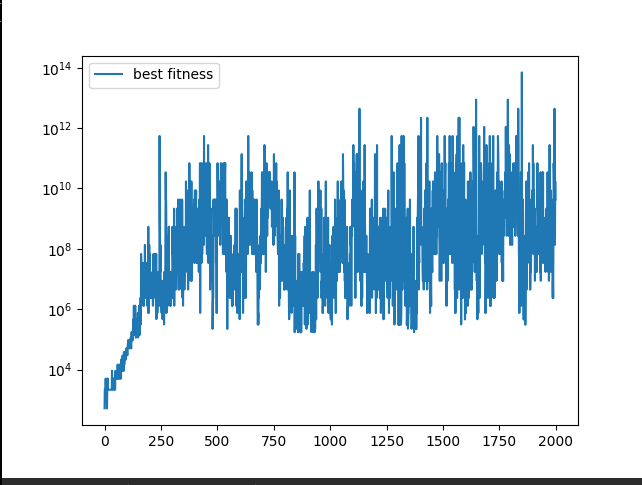
\includegraphics[width=0.8\textwidth]{bf}
\caption{Analiza optymalnego węża w zależności od pokolenia, 2000 pokoleń}
\end{figure}
\begin{figure}[H]
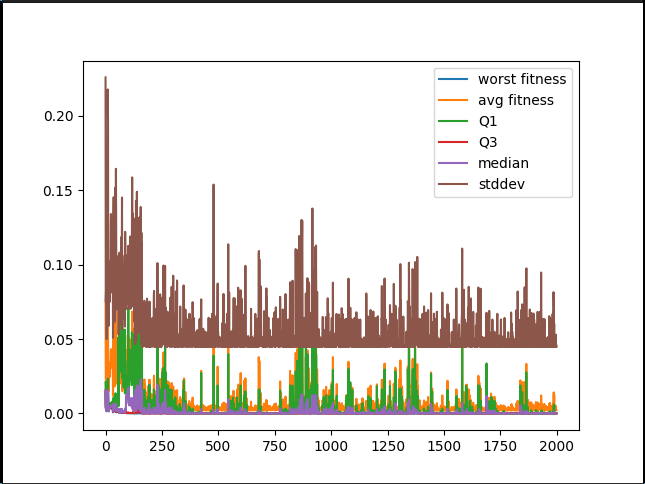
\includegraphics[width=0.8\textwidth]{stat}
\caption{Analiza statystyczna całego pokolenia}
\end{figure}

\section{Wnioski} 
Po wyszkoleniu węża na małej mapie, na której rozgrywki są szybsze, przenieśliśmy ten sam algorytm na mapę większą (bez dalszego szkolenia). Co ciekawe, wyszkolone węże radziły sobie stosunkowo dobrze.
\section{Bibliografia}
Kumar, Rakesh & Jyotishree,. (2012). Blending Roulette Wheel Selection & Rank Selection in Genetic Algorithms. International Journal of Machine Learning and Computing. 365-370. 10.7763/IJMLC.2012.V2.146.  \\
J. D. Schaffer, D. Whitley and L. J. Eshelman, "Combinations of genetic algorithms and neural networks: a survey of the state of the art," [Proceedings] COGANN-92: International Workshop on Combinations of Genetic Algorithms and Neural Networks, Baltimore, MD, USA, 1992, pp. 1-37, doi: 10.1109/COGANN.1992.273950. \\
Seyedali Mirjalili - Evolutionary Algorithms and Neural Networks. Theory and Applications-Springer (2019) \\
David J. Montana and Lawrence Davis. 1989. Training feedforward neural networks using genetic algorithms. In Proceedings of the 11th international joint conference on Artificial intelligence - Volume 1 (IJCAI'89). Morgan Kaufmann Publishers Inc., San Francisco, CA, USA, 762–767. \\
Whitley, Darrell. (1998). Genetic Algorithms and Neural Networks. \\
\end{document}
